\documentclass[border=0mm]{standalone}
\usepackage{pgfplots}
\usepgfplotslibrary{groupplots}
\pgfplotsset{compat=1.17}
\usepackage{xcolor}
\usepackage{xstring}

\newcommand{\Tukeywindow}[3]{% beta, delay, color
\addplot[#3, samples=200, thick] {func(x-#2,#1)};
}




\begin{document}

\pgfplotsset{
compat=1.11,
legend image code/.code={
\draw[mark repeat=2,mark phase=2]
plot coordinates {
(0cm,0cm)
(0.15cm,0cm)        %% default is (0.3cm,0cm)
(0.3cm,0cm)         %% default is (0.6cm,0cm)
};%
}
}

\definecolor{lightblue}{RGB}{86,192,150}  % Define light blue color

\pgfdeclarelayer{background layer}
\pgfdeclarelayer{foreground layer}
\pgfsetlayers{background layer,main,foreground layer}

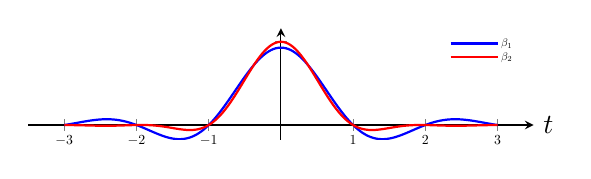
\begin{tikzpicture}[
declare function={
	sinc(\x) = (\x == 0) * 1+
			(\x!=0) * sin(pi*deg(\x))/(pi*\x) ;
	cosc(\x,\b)= or(x==1/(2*\b),x==-1/(2*\b)) * pi/4 +
			and(x!=1/(2*\b),x!=-1/(2*\b)) * cos(deg(pi*\x*\b))/(1-(2*\b*\x)^2);
	func(\x,\b) = 2/sqrt(4-\b)*sinc(\x)*cosc(\x,\b);
},
]
\begin{axis}[
  width = 8cm,
  height = 3cm,
  xlabel={$t$},
  axis x line=middle,  % Show only the x-axis
  axis y line=middle,    % Hide the y-axis
  xmin=-3.5, xmax=3.5,
  ymin=-0.2, ymax=1.3,  % Set ymax to 2
  xtick={-3,-2,...,3},
  ytick={2/sqrt(4-0.8),2/sqrt(4-0.3)},
  yticklabels=\empty,
  every tick label/.append style={scale=0.5},
  xlabel style={
    right,
  },
  legend style={draw=none,nodes={scale=0.4, transform shape}}
]

\Tukeywindow{0.3}{0}{blue, domain = -3:3}
\addlegendentry{$\beta_1$}
\Tukeywindow{0.8}{0}{red, domain = -3:3}
\addlegendentry{$\beta_2$}

\end{axis}


\end{tikzpicture}

\end{document}
























